\documentclass[11pt]{article}
%%%%%%%%%%%%%%%%%%%%%%%%%%%%%%%% Algunos Paquetes Necesarios 
\usepackage{fancyhdr, graphicx}
\usepackage[utf8]{inputenc} % Tildes
\usepackage[spanish]{babel} % Language
\usepackage{babelbib} % Bibliografia español
\usepackage[margin=1in]{geometry} % Margins														
\usepackage{amssymb}
\usepackage{amsmath, amsthm, amsfonts}
\usepackage[table]{xcolor} % Color table
\usepackage{longtable} % Table accross multiple pages
\usepackage{hyperref}  % Use Hyperlinks
\usepackage{enumitem} % Reduce space in enumerate
\usepackage{multicol}
\usepackage{tkz-euclide}
%\usetkzobj{all}
\decimalpoint




\begin{document} %%%%%%%%%%%%%%%%%%%%%%%% BEGIN%%%%%%%%%%%%%%


%%%%%%%%%%%%%%%%%%%%%%%%%%%%%%%%% Titulo
{\color{white}.}
\vspace{3 in}
\begin{center}
\Huge

\textsc{MAP 1  $-$ Curvas de Bézier  %NOMBRE_MAP
}
\\
\textsc{Reporte}

\end{center}
%%%%%%%%%%%%%%%%%%%%%%%%%%%%%%%%% Titulo


\vspace{3 in}
\hrule height 1.5pt
\vspace{0.1 in}

%%%%%%%%%%%%%%%%%%%%%%%%%%%%%%%%% Datos Grupo
{\large
\noindent \textbf{Integrantes: } 
\begin{itemize}[nolistsep]
	\item José Roberto Sosa Zamora $-$ $20004225$.
	\item Alejandra Nazareth Sosa Carrillo$-$ $22002246$.
 \end{itemize}

}
\vspace{0.2 in}
\hrule height 1.5pt

\newpage
\vspace{0.1 in}
%%%%%%%%%%%%%%%%%%%%%%%%%%%%%%%%% Datos Grupo - END


%%%%%%%%%%%%%%%%%%%%%%%%%%%%%%%%% MAP
\begin{center}
	\Large	
	\textbf{MAP 1 Curvas de Bézier }
\end{center}

\noindent \textbf{Parte I }

		\begin{itemize}
			\item[$1)$]Grafique la curva de Bézier generada por puntos de control $P_{0}(4, 1), P_{1}(28, 48), P_{2}(50, 42)$  y $ P_{3}(40, 5).$
		\begin{figure}[h]
		
				\[
				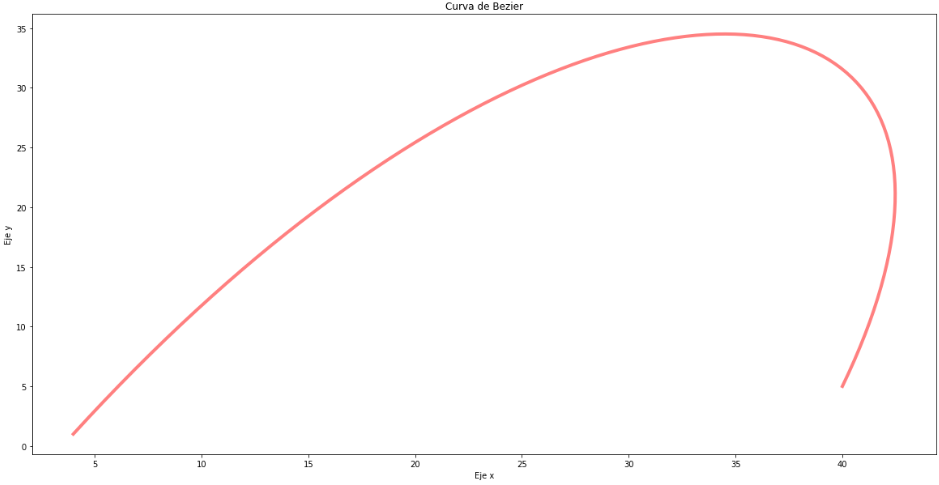
\includegraphics[scale=0.5]{graphs/bezier_graph.png }
				\]
				\caption{Curva de Bézier generada por puntos de control $P_{0}(4, 1), P_{1}(28, 48), P_{2}(50, 42)$  y $ P_{3}(40, 5).$}
		\end{figure}
				

	\[
	%% EJEMPLO DE ECUACION CENTRADA
	x(t)=t^2+ \displaystyle \frac{t}{2} 
	\]
	\[
	%% EJEMPLO DE ECUACION CENTRADA
	x = x_{0}\,(1 - t )^3 \,+ \,3x_{1} \, t(1 - t)^2 \, + \, 3x_{2} \, t^2(1-t) \,+ \, x_{3}t^3
	\]	\[
	%% EJEMPLO DE ECUACION CENTRADA
	y = y_{0}\,(1 - t )^3 \,+ \,3y_{1} \, t(1 - t)^2 \, + \, 3y_{2} \, t^2(1-t) \,+ \, y_{3}t^3
	\]

	\item[$2)$]  En la misma gráfica, trace los segmentos de recta $\overline{P_{0}P_{1}}, \overline{P_{1}P_{2}}$ y $\overline{P_{2}P_{3}}$. 
		         Notar como los puntos de control medio  no están sobre la curva. La curva inicia en $P_{0}$, se dirige hacia $P_{1}$ y $P_{2}$ 
		         sin alcanzarlos y termina en $P_{3}$. 
						
			\begin{figure}[h]
			
					\[
					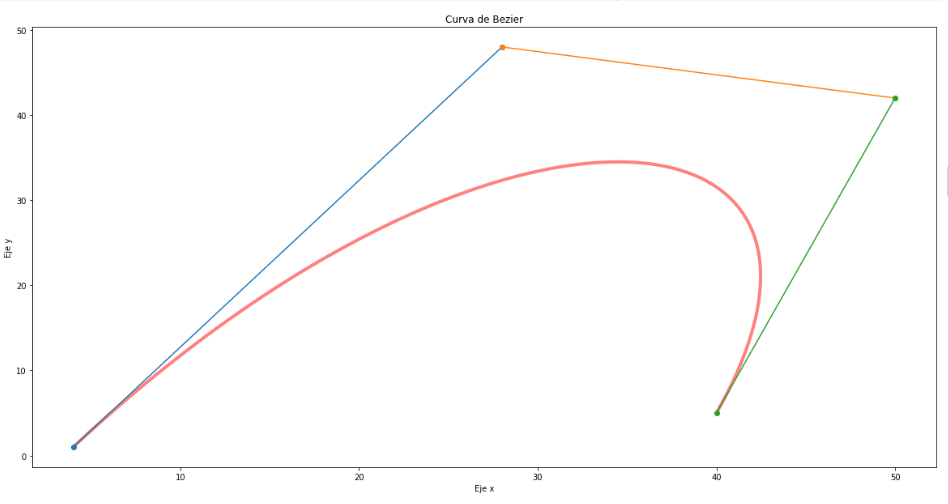
\includegraphics[scale=0.5]{graphs/line_segments.png }
					\]
					\caption{segmentos de recta $\overline{P_{0}P_{1}}, \overline{P_{1}P_{2}}$ y $\overline{P_{2}P_{3}}$.}
			
			\end{figure}



 %Ejemplo ecuacion no centrada


	\item[$3)$] Algunas impresoras láser usan las curvas de Bézier para representar letras y otros símbolos.
  		        Experimente con puntos de control hasta que encuentre una curva de Bézier que dé una
		         representación razonable de la letra C.
		        \begin{figure}[h]
			
					\[
					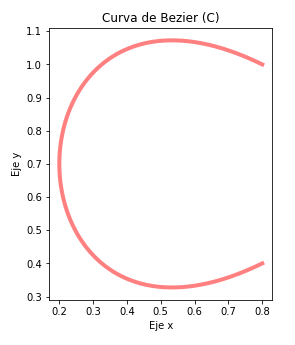
\includegraphics[scale=0.8]{graphs/graph_C.png }
					\]
					\caption{representación de curva de Bézier de la letra C de segmentos de rectas $\overline{P_{0}P_{1}}, \overline{P_{1}P_{2}}$ y $\overline{P_{2}P_{3}}$.}
			
			\end{figure}

	\item[$4)$] Se pueden representar formas más complicadas al unir dos o más curvas de Bezier. Suponga
		        que la primera curva de Bézier tienen puntos de control P0, P1, P2 y P3 y la segunda tiene 
		       Puntos de control P3, P4, P5 y P6. Sí desea unir estos dos trozos de manera “suave”,
  		       entonces las rectas tangentes en P3 debe corresponderse y, por tanto, los puntos P2, P3 y P4
		       tiene que estar sobre esta recta tangente común. 

		      Grafique las curvas de Bézier que considere necesarias para escribir el nombre o apellido de
		       algún matemático famoso (con un mínimo de 6 letras). No olvide agregar dichas ecuaciones
  		       y su gráfica al reporte



\end{itemize}
\noindent \textbf{Parte II }
\begin{enumerate}
	\item
	\item
	\item
\end{enumerate}


\begin{center}
	\Large	
	\textbf{Referencias }
\end{center}
\begin{itemize}
	\item
	\item
\end{itemize}

\end{document} %%%%%%%%%%%%%%%%%%%%%%%% BEGIN%%%%%%%%%%%%%%